%-------------------------------------------
\begin{frame}{
\includegraphics[height=0.8cm]{shared/logo-github.png}}
%-------------------------------------------
\begin{exampleblock}{Previous exercise}
In the previous exercise, we added change in the fork of our GitHub account through the GitHub GUI.
\end{exampleblock}
\begin{exampleblock}{Objective}
Now we will again modify a file but using a local working copy, so that we can work independently of the internet connection.\\
We will also collaborate all together (eg. the final README.md file should contains the name of all of us) \\
\vfill
Steps of modifications will be done with git on a local clone while steps for collaborative building will be done through the GitHub interface.
\end{exampleblock}
\end{frame}
%-------------------------------------------
\begin{frame}[containsverbatim]
\frametitle{\raisebox{-1ex}{
\includegraphics[height=0.8cm]{shared/logo-github.png}}}
%-------------------------------------------
\begin{exampleblock}{Repository to fork:}
We could use the previous forked repository to do the collaborative part, but as we want to practice changes in a local copy, we will fork another repository: \href{https://github.com/clairetn/FAIR_bioinfo_github.git}{\textcolor{blue}{clairetn, \underline{FAIR$\_$bioinfo$\_$github}}}
\end{exampleblock}
\begin{exampleblock}{Be added as collaborator to the repository}
To work in a collaborative mode we will invite our neighbors as collaborator in the Settings tab of this repository: need to exchange our github login.
\end{exampleblock}
\end{frame}
%-------------------------------------------
\begin{frame}[containsverbatim]
\frametitle{\raisebox{-1ex}{
\includegraphics[height=0.8cm]{shared/logo-github.png}}}
%-------------------------------------------
\begin{exampleblock}{Steps}
\begin{enumerate}
    \item fork the repository on your github account (github fork)
    \item invite your left and right neighbors to collaborate in your fork
    \item clone your own forked repository in a new local working repository (git, local)
    \item create a new branch (git, local)
    \item do the modification (add your name in the README.md file) (local)
    \item merge the branch (git local)
    \item push the actual local version to our github repository (git local)
    \item pull request the original github repository of our changing (github)
    \item as a collaborator, push your changing in the original upstream repository (github)
\end{enumerate}
\end{exampleblock}
\end{frame}
%-------------------------------------------
\begin{frame}[containsverbatim]
\frametitle{\raisebox{-1ex}{
\includegraphics[height=0.8cm]{shared/logo-github.png}}: Cloning one of your fork}
%-------------------------------------------
\begin{exampleblock}{Github url:}
\begin{columns}
\column{0.5\textwidth}
\begin{itemize}
    \item We clone a fork with the git command \verb|git clone| followed by the url of the repository.
    \item This url is accessible with our mouse from the github repository (green "Code" button):
\end{itemize}
\column{0.45\textwidth}
\begin{center}
    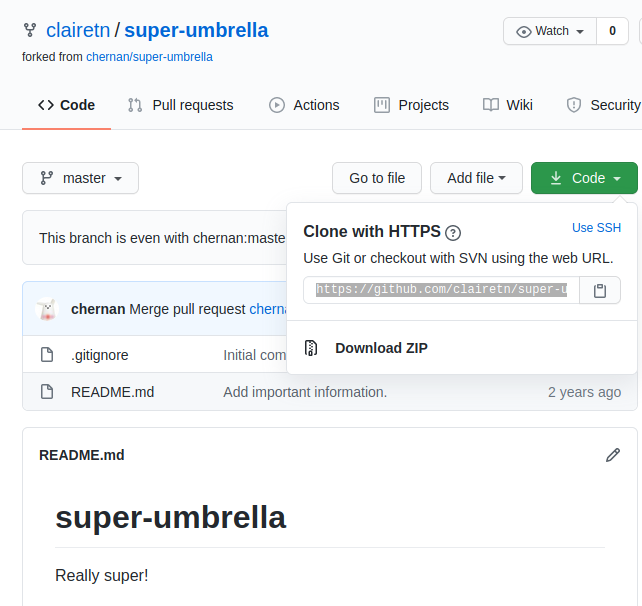
\includegraphics[height=5cm]{05_history/Images/FAIR_github_clone.png}
\end{center}
\end{columns}
\begin{center}
    \small{\verb|https://github.com/clairetn/FAIR_bioinfo_github.git|}
\end{center}
\end{exampleblock}
\end{frame}
%-------------------------------------------
\begin{frame}[containsverbatim]
\frametitle{\raisebox{-1ex}{
\includegraphics[height=0.8cm]{shared/logo-github.png}}: Git commands}
%-------------------------------------------
\begin{exampleblock}{GUI Github $\rightarrow$ local git (just done):}
\begin{lstlisting}
git clone <url_of_your_github_account>
\end{lstlisting}
\end{exampleblock}
\begin{exampleblock}{Local work:}
\begin{lstlisting}[language=python]
git branch mybranch
git checkout mybranch
# do change, eg. add your name in README.md file
git add README.md
git commit -m "add name"
git checkout master
git merge mybranch
git delete mybranch
\end{lstlisting}
\end{exampleblock}
\begin{exampleblock}{Local git $\rightarrow$ GUI Github:}
\begin{lstlisting}
git push origin master
\end{lstlisting}
\end{exampleblock}
\end{frame}
%-------------------------------------------
\begin{frame}[containsverbatim]
\frametitle{\raisebox{-1ex}{
\includegraphics[height=0.8cm]{shared/logo-github.png}}: Propose your change into the initial project}
%-------------------------------------------
\begin{exampleblock}{From your forked repository} 
\begin{itemize}
    \item "Compare" and then "Pull request" your issue (explain your proposals as much as possible)
    \item conflicts when one change the same line 
    \item manage possible conflicts with the Github GUI
\end{itemize}
\end{exampleblock}
\begin{exampleblock}{Many small commits} 
$\Rightarrow$ do many small commits easier to merge than a big unique one
\end{exampleblock}
\end{frame}
%-------------------------------------------
\begin{frame}{Bonus}
%-------------------------------------------
\begin{exampleblock}{Challenge}
\begin{itemize}
    \item make a (voluntary today) "error" by suppressing the new dedicated repository created for this git exercise
    \item retrieve your code with the git clone command on your github repository
\end{itemize}
\end{exampleblock}
\end{frame}